%========================================================================
% Modelo para elaboracao de textos academicos: TCC, dissertacoes e teses
% Elaborado pelo GISIS - Grupo de Imageamento Sismico e Inversao Sismica.
%========================================================================
\chapter{Discussões}
\label{ch:discussoes}

% Focar nos impactos da imprecisão no cálculo dos tempos na inversão
% Analisar as diferenças e ruídos de inversão para cada método
% Analisar performance em relação aos resultados
 
\begin{figure}[H]
	\centering
	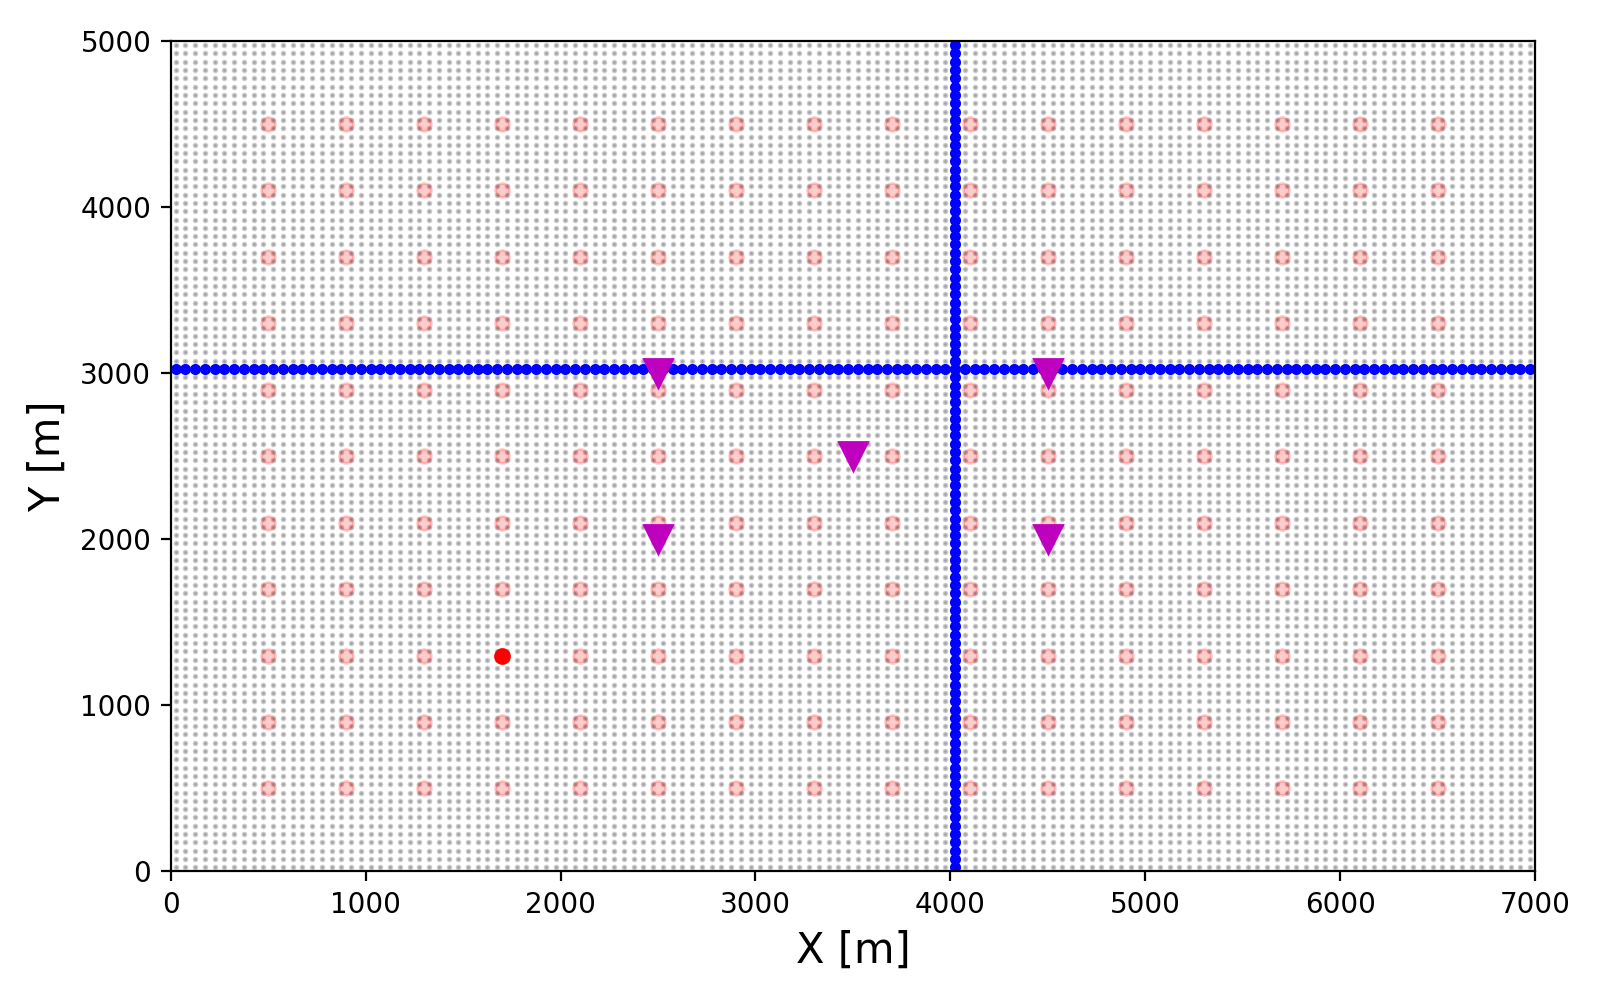
\includegraphics[width=12cm,height=7cm]{Imgs/Discussoes/discuss_geometry.png}
	\caption{Panorama de discussão envolvendo o dado e os modelos. Em relação aos dados, que estão ordenados no domínio do receptor, o ponto vermelho de tonalidade marcante será o receptor de referência. Os pontos azuis em destaque são as linhas de tiros utilizadas apara a análise. Em relação ao modelo, cinco pontos foram destacados nas mesmas posições das gaussianas utilizadas para gerar o modelo de referência.}
	\label{fig:discuss_geometry}	
\end{figure}

\begin{figure}[H]
	\centering
	\subfloat[]{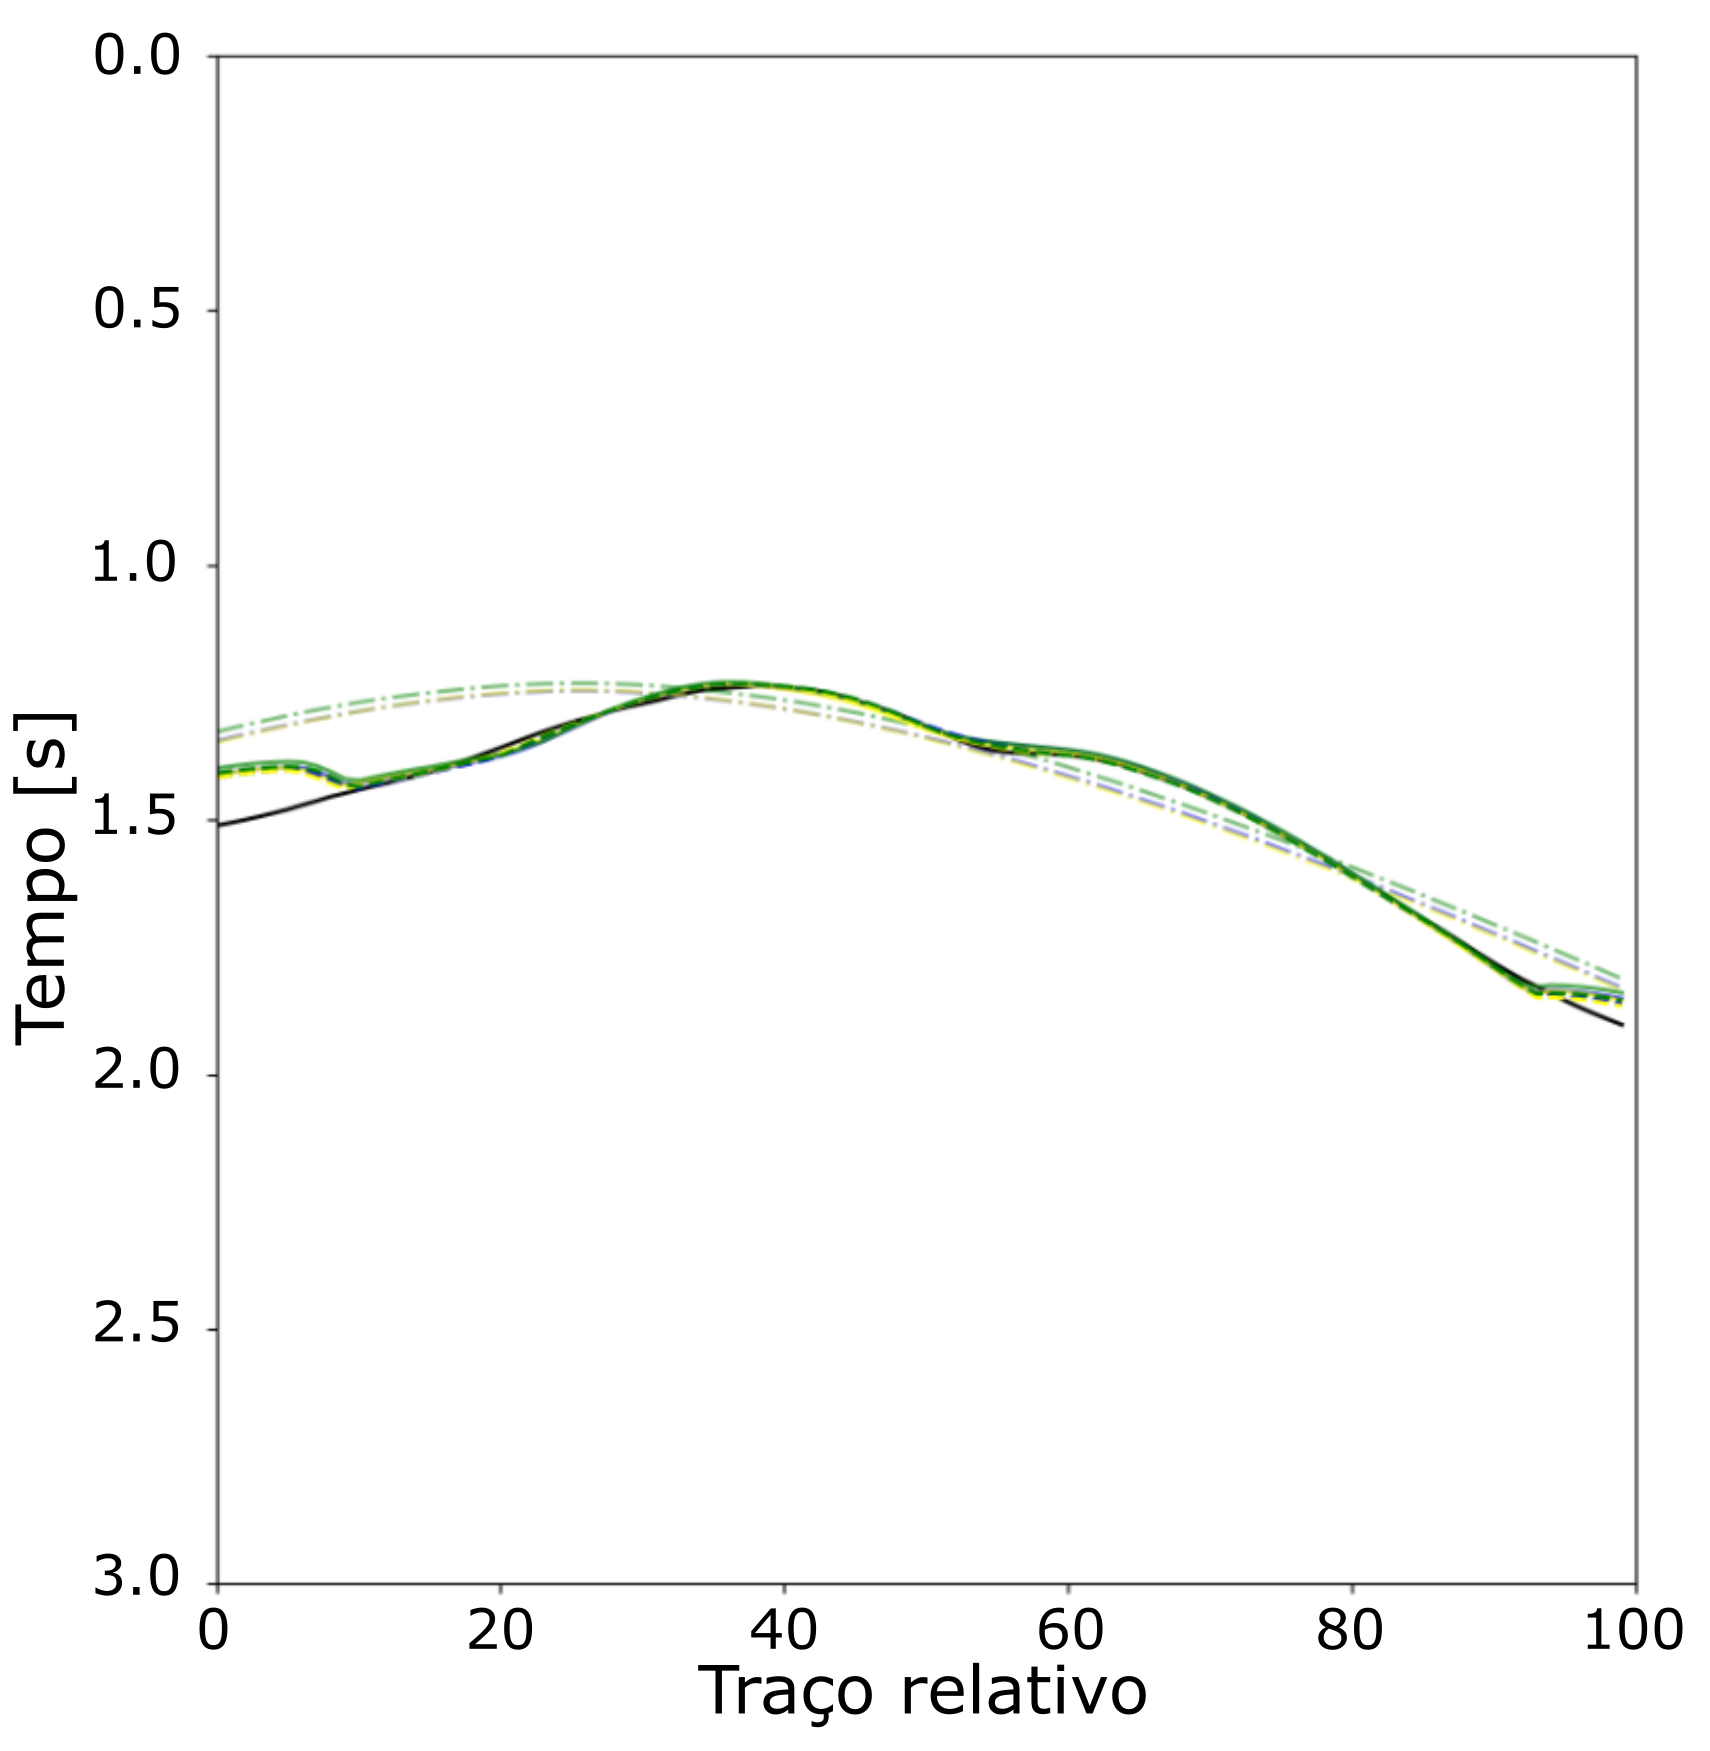
\includegraphics[width=8cm,height=8cm]{Imgs/Discussoes/xz_zoom_out.png}}
	\subfloat[]{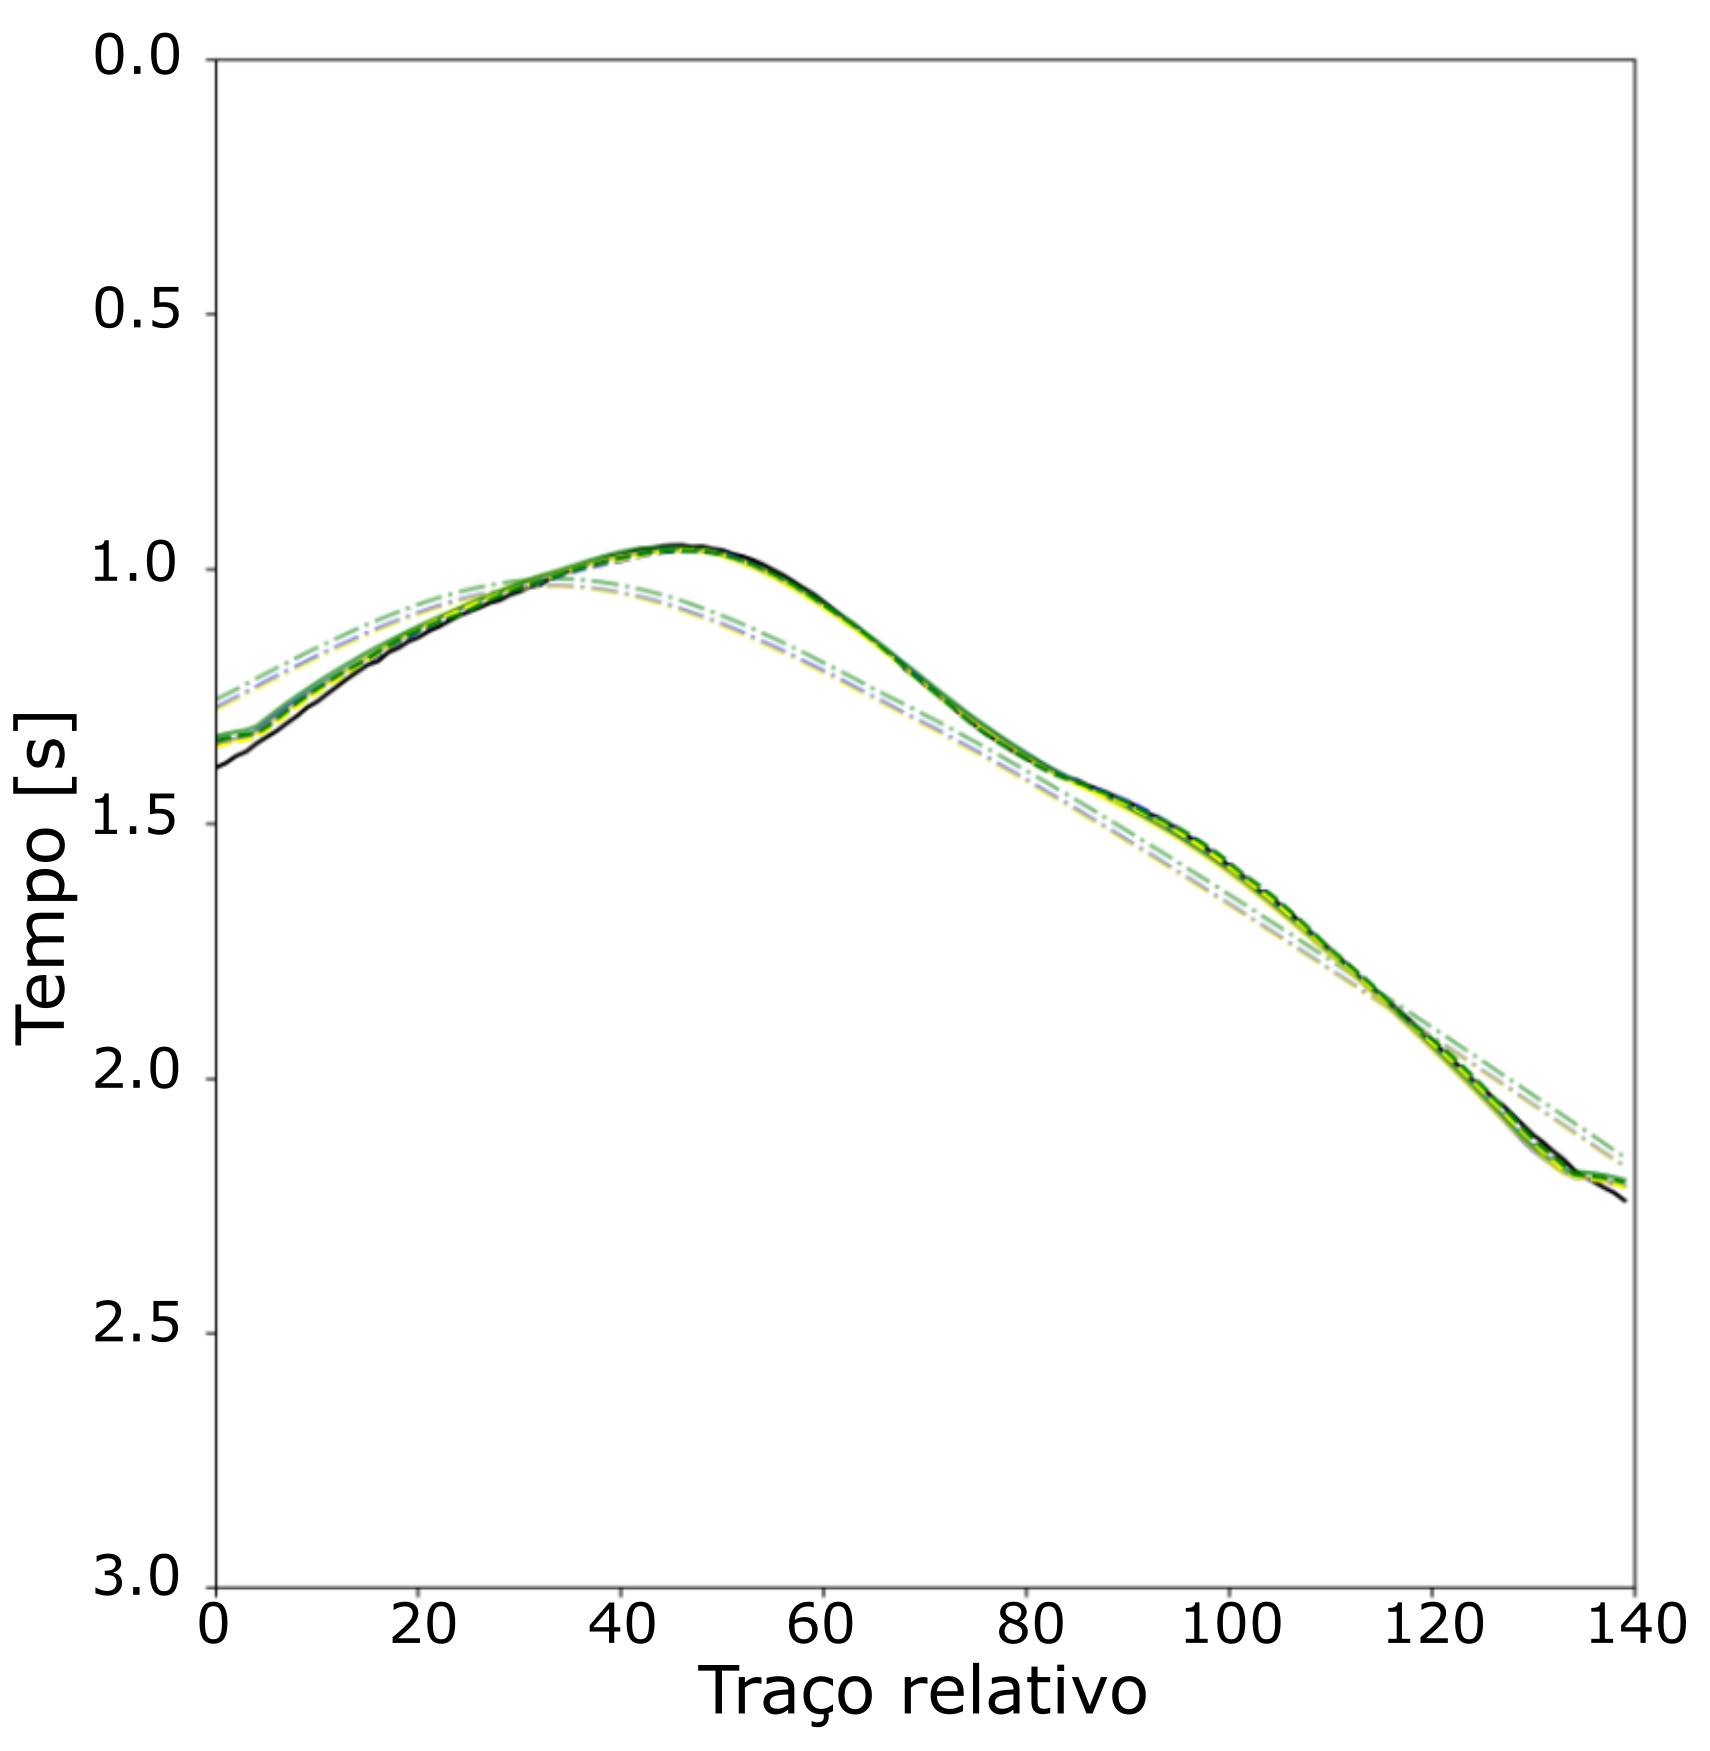
\includegraphics[width=8cm,height=8cm]{Imgs/Discussoes/yz_zoom_out.png}}
	
	\caption{Comparação de dados incluindo o dado observado, linha preta sólida, dado inicial, linhas coloridas com traço e ponto, dado gerado a partir do primeiro processo de inversão, linhas coloridas sólidas, e o dado gerado a partir do segundo processo de inversão, linhas coloridas tracejadas. Em relação aos métodos estudados, a cor azul se refere à formulação de \citeonline{podvin1991finite}, a cor amarela \citeonline{jeong2008fast} e a cor verde \citeonline{jeong2008fast}.}
	\label{fig:zoom_out}
\end{figure}

\begin{figure}[H]
	\centering
	\subfloat[]{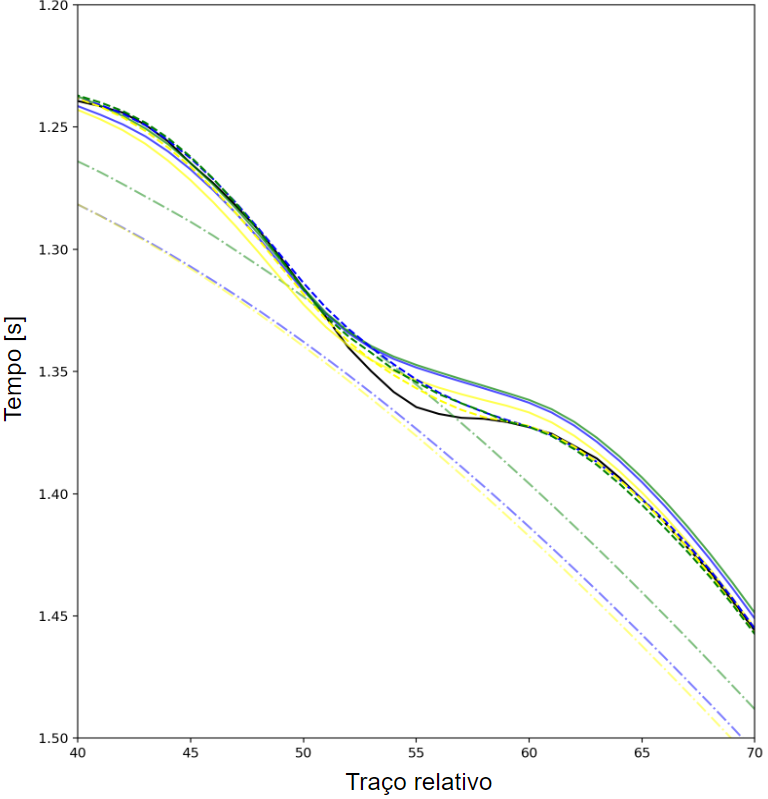
\includegraphics[width=8cm,height=8cm]{Imgs/Discussoes/xz_zoom_in.png}}
	\subfloat[]{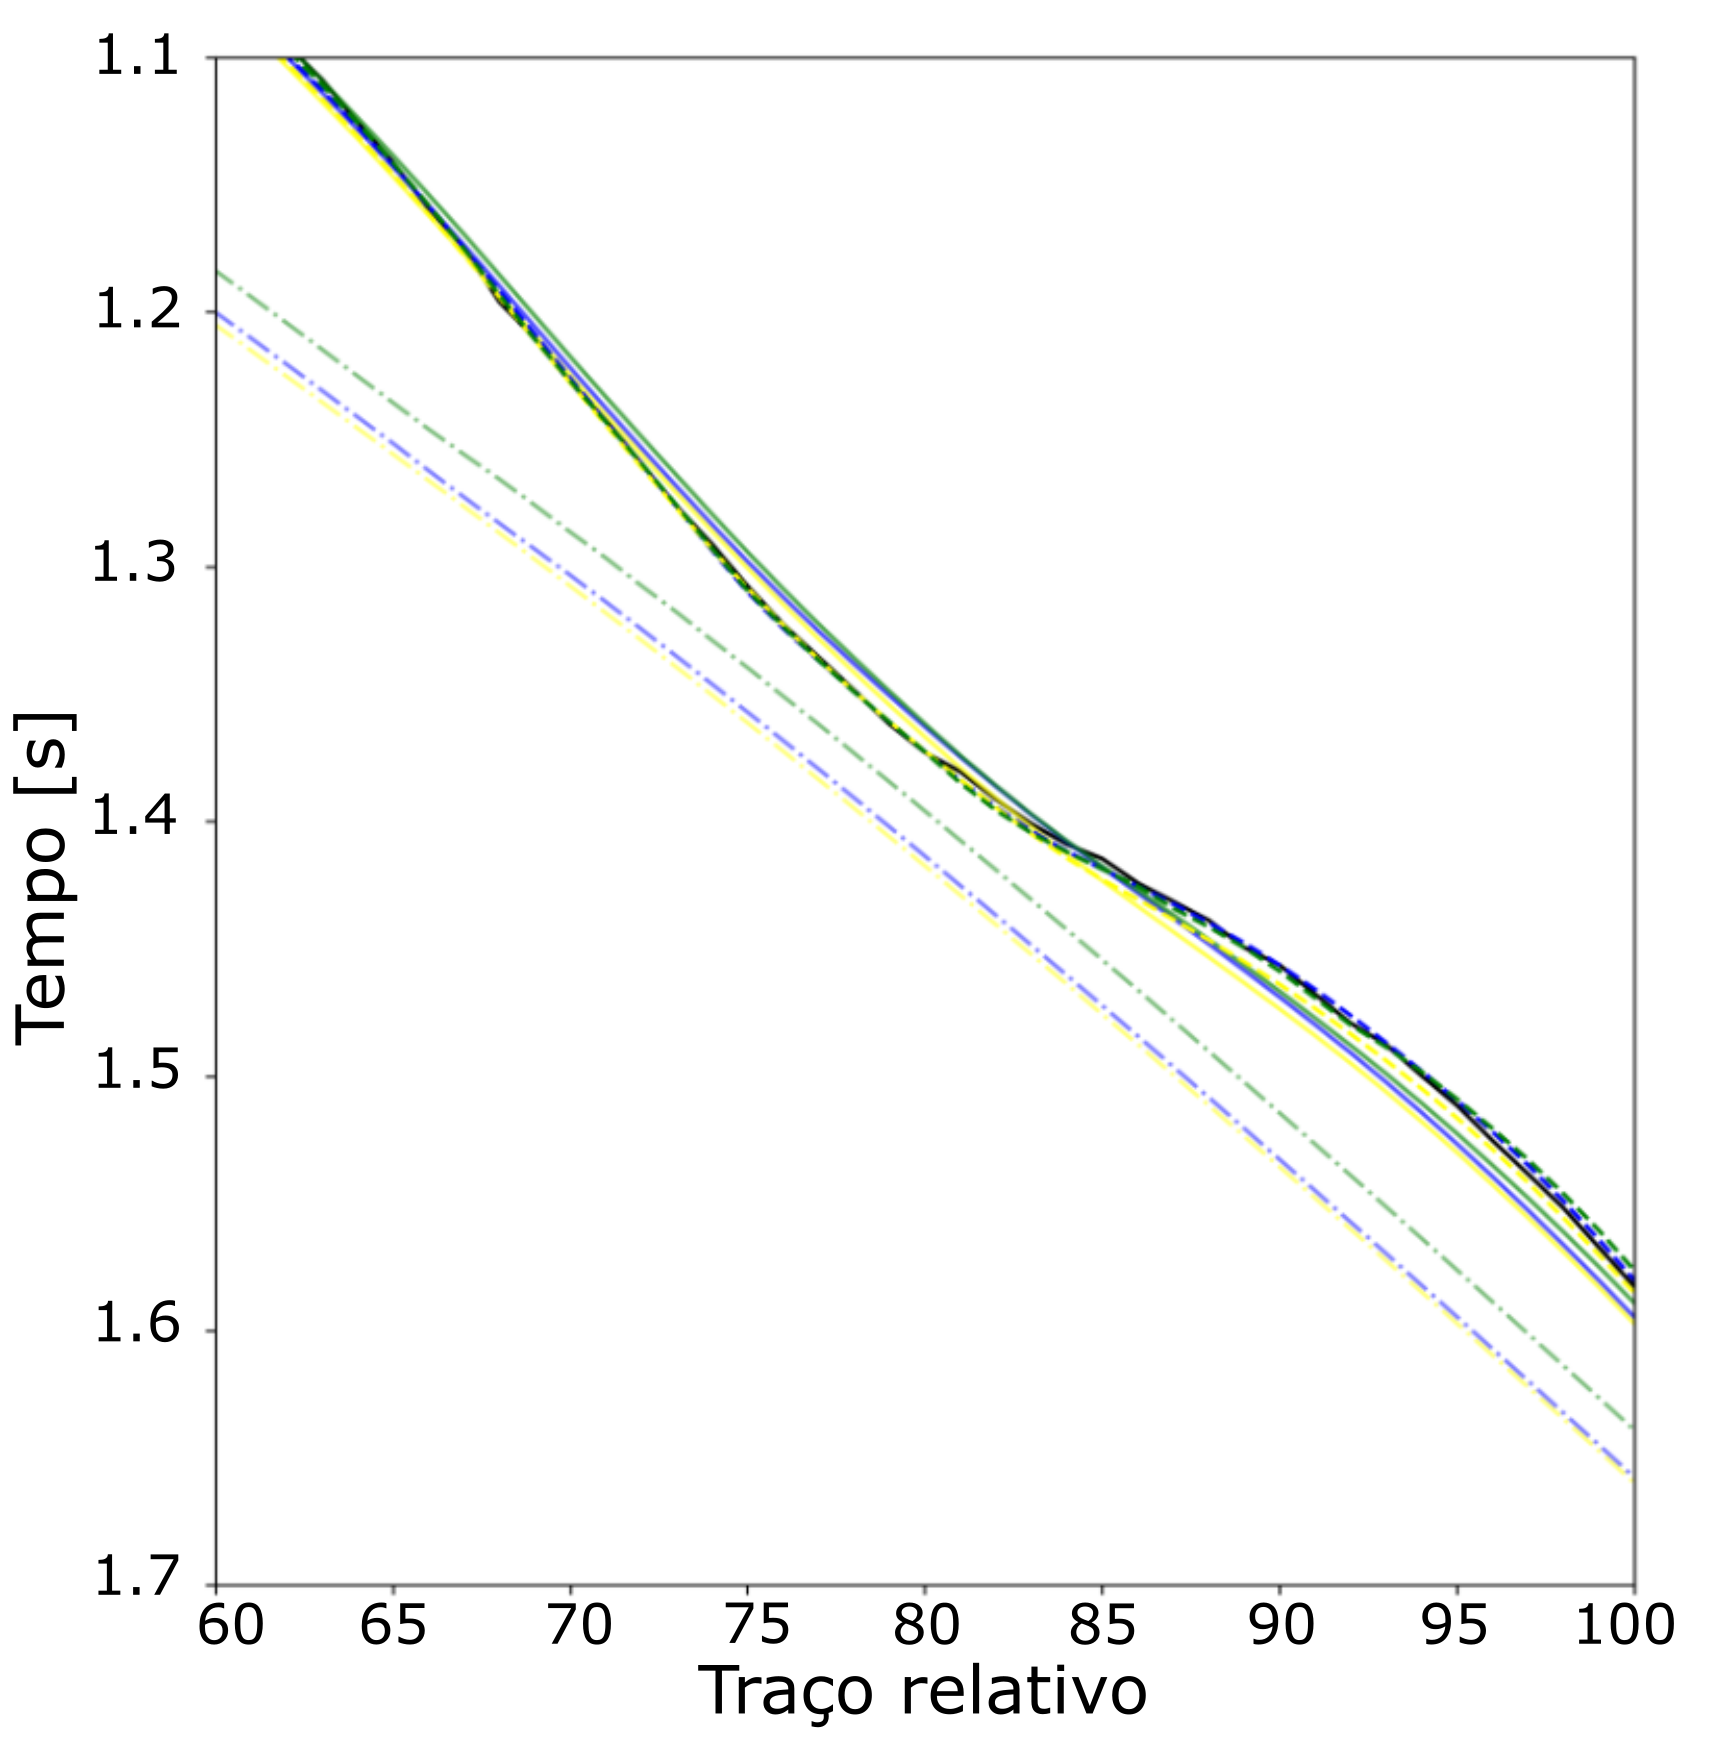
\includegraphics[width=8cm,height=8cm]{Imgs/Discussoes/yz_zoom_in.png}}
	
	\caption{Aproximação para melhor analise dos dados. Dado observado se apresenta como a linha preta sólida, o dado inicial, linhas coloridas com traço e ponto, dado gerado com modelo da inversão esparsa, linhas coloridas sólidas, e o dado gerado com modelo da inversão refinada, linhas coloridas tracejadas. Em relação aos métodos estudados, a cor azul se refere à formulação de \citeonline{podvin1991finite}, a cor amarela \citeonline{jeong2008fast} e a cor verde \citeonline{jeong2008fast}.}
	\label{fig:zoom_in}
\end{figure}


\begin{figure}[H]
	\centering
	\subfloat[]{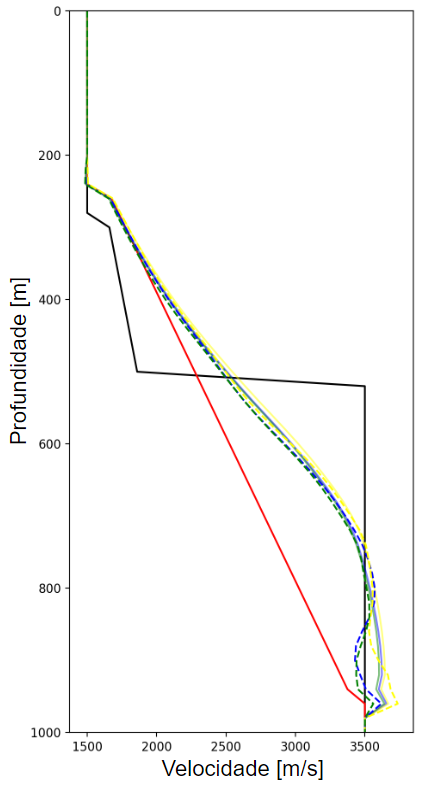
\includegraphics[width=3.2cm,height=6cm]{Imgs/Discussoes/upper_left_corner.png}}
	\subfloat[]{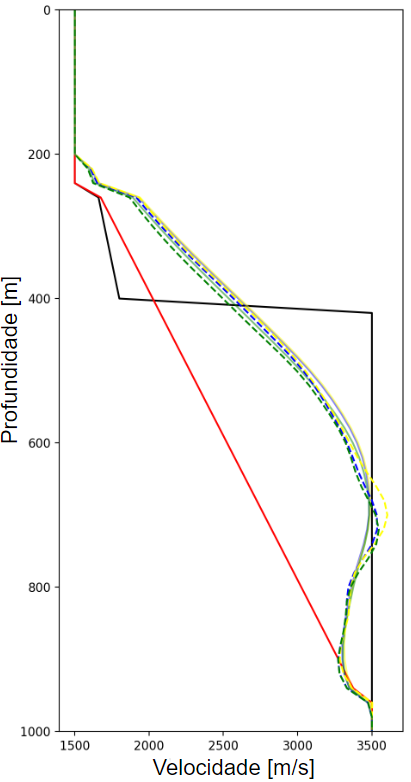
\includegraphics[width=3.2cm,height=6cm]{Imgs/Discussoes/lower_left_corner.png}}
	\subfloat[]{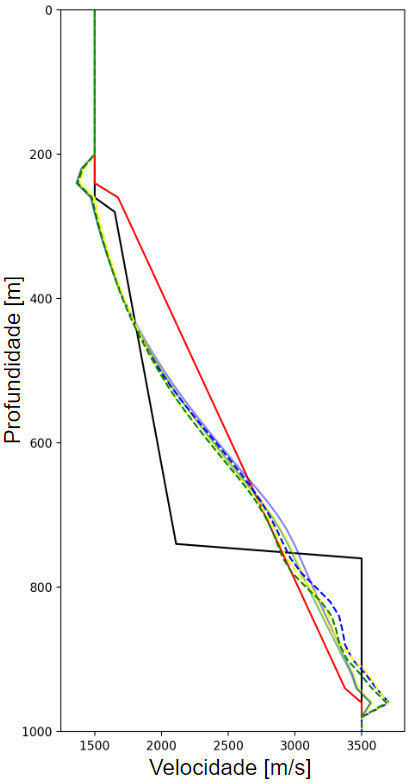
\includegraphics[width=3.2cm,height=6cm]{Imgs/Discussoes/center.png}}
	\subfloat[]{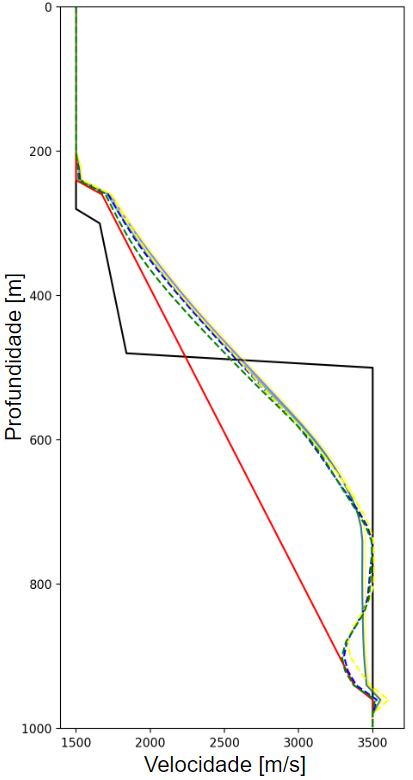
\includegraphics[width=3.2cm,height=6cm]{Imgs/Discussoes/upper_right_corner.png}}
	\subfloat[]{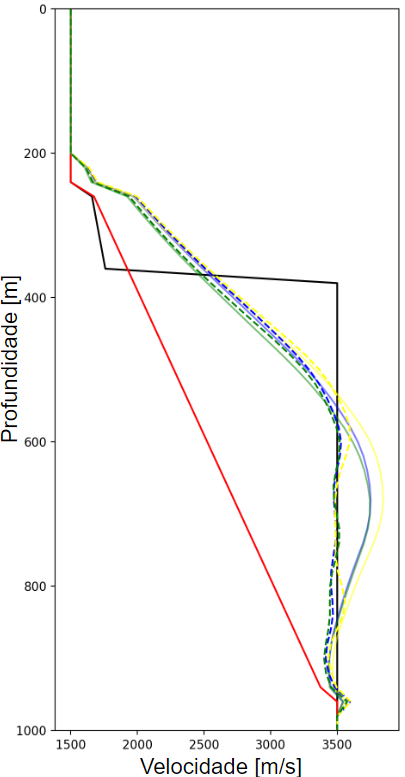
\includegraphics[width=3.2cm,height=6cm]{Imgs/Discussoes/lower_right_corner.png}}
	
	\caption{Modelos finais em forma de traço em cada posição central das gaussianas utilizadas. (a) Modelos projetados no ponto superior esquerdo. (b) Projeção no ponto inferior esquerdo. (c) Projeção central. (d) Projeção no ponto superior direito. (e) Projeção no ponto inferior direito. Em relação às cores, o modelo de referência se apresenta como o traço preto sólido e o modelo inicial como o traço vermelho sólido. Traços coloridos sólidos se referem aos modelos recuperados com malha esparsa e traços coloridos tracejados são modelos recuperados com malha refinada. Os métodos estudados recebem as cores: azul para \citeonline{podvin1991finite}, amarela para \citeonline{jeong2008fast} e verde para \citeonline{jeong2008fast}.}
	\label{fig:}
\end{figure}



